\documentclass[12pt]{article}
\usepackage[a4paper, portrait, margin=1cm, right=1cm]{geometry}
\usepackage{fontspec}
\usepackage[fleqn]{amsmath}
\usepackage{setspace}
\usepackage{graphicx}
\graphicspath{./graphics/}
\setmainfont[Ligatures=TeX]{Linux Libertine}

\title{АиГ. ДЗ к 12.10.2022. Вариант №13}
\author{Студент группы 2305 Александр Макурин}
\date{30 сентября 2022}

\begin{document}

\maketitle

\begin{sloppypar}
    \setstretch{1.8}

    \section{Решите уравнение $3x^2 - 5x + 8 = 0$.}
    $
        3x^2-5x+8=0 \\
        D = (-5)^2 - 4*3*8 = 25 - 96 = -71 \\
        x_{1,2} = \dfrac{5 \pm \sqrt{-71}}{6} = \dfrac56 \pm \dfrac{i\sqrt{71}}{6}
    $

    \framebox{Ответ:  $x_{1,2} = \dfrac56 \pm \dfrac{i\sqrt{71}}{6}$}

    \section{Выполните действия $i^{15}(7 + i) + \dfrac{-5 + i}{-1 + i}$.}
    $
        i^{15}(7+i) + \dfrac{-5 + i}{-1 + i} = 1 - 7i + \dfrac{-5 + i}{-1 + i} = \\
        = \dfrac{-1 + i + 7i + 7 - 5 + i}{-1 + i} = \dfrac{1 + 9i}{-1 + i} = \dfrac{-1 - 9i + i - 9}{1 - 2i - 1} = \\
        = \dfrac12i(-10 - 8i) = 4 - 5i
    $

    \framebox{Ответ: $4 - 5i$}

    \section{Решить в алгебраической форме: $z^2 + (8 - i)z + 14 + 2i = 0$}
    $
        z^2 + (8 - i)z + 14 + 2i = 0 \\
        a = 1 \\
        b = 8 - i \\
        c = 14 + 2i \\
        D = (8 - i)^2 - 4(14 + 2i) = 63 - 16i - 56 - 8i = 7 - 24i \\
        z_{1,2} = \dfrac{i - 8 \pm \sqrt{7 - 24i}}{2} \\
        \sqrt{7 + (-24i)} = a + bi \\
        \left\{
        \begin{array}{ll}
            a^2 - b^2 = 7 \\
            2ab = -24 \Rightarrow a = -\dfrac{12}b
        \end{array}
        \right .
        \\
        \dfrac{144}{b^2} - b^2 = 7 \hspace{10pt}| *b^2 \\
        144 - b^4 = 7b^2 \\
    $Пусть $ t = b^2, t \geq 0 \\
        t^2 + 7t - 144 = 0 \\
        D = 49 + 4 \cdot 144 = 625 \\
        t_{1,2} = \dfrac{-7 \pm \sqrt{625}}{2} = -16, 9 \\
        -16 < 0 \Rightarrow t = 9 \Rightarrow
        \left|
        \begin{array}{ll}
            b_{1,2} = \mp 3 \\
            a_{1,2} = \pm 4
        \end{array}
        \right . \\
        \sqrt{7 + (-24i)} = \pm(4 - 3i) \\
        z_{1,2} = \dfrac{i - 8 \pm (4 - 3i)}{2} = \dfrac{-4 - 2i}{2}, \dfrac{-12 + 4i}{2} = -2 - i, -6 + 2i
    $

    \framebox{
        Ответ: $z_{1,2}= \left|
            \begin{array}{cc}
                -6 + 2i \\
                -2 - i
            \end{array}
            \right .$
    }

    \section{
      Изобразите множество точек на комплексной плоскости, удовлетворяющих
      $\left\{
          \begin{array}{ll}
              |z + 3 + 2i| > 5 \\
              \text{Re } z \geq -1
          \end{array}
          \right .$
     }
    $
        |z + 3 + 2i| > 5 \\
        |z - (-3 - 2i)| > 5 \\
        |z - z_0| = R - \text{окружность}
    $
    \\
    \framebox{\textsc{Ответ: }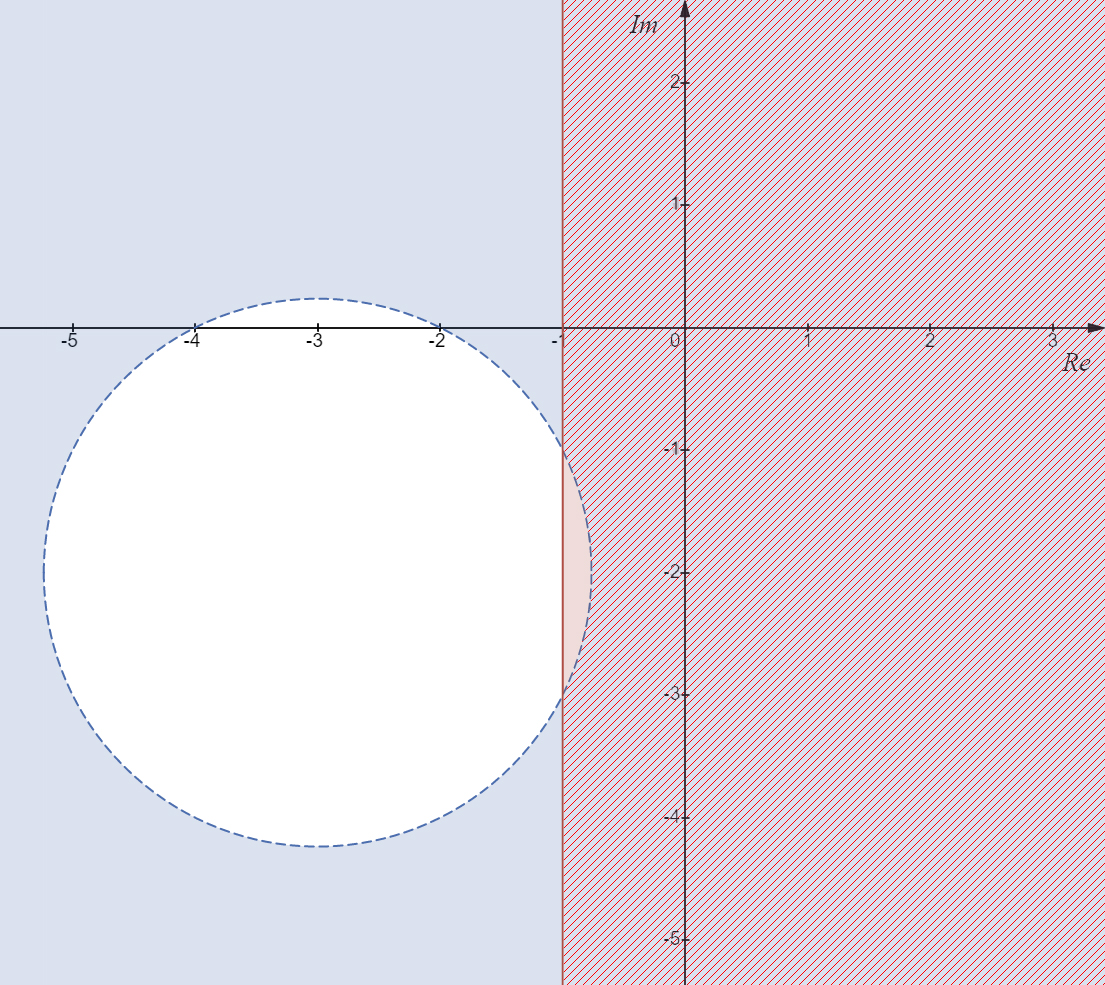
\includegraphics[width=0.8\textwidth]{graphics/ИДЗ1_Вариант13_график.jpg}}

    \section{Найдите все значения $\sqrt[3]{-216 + 216i}$. Ответ запишите в показательной форме}
    $
        \sqrt[3]{-216 + 216i} = \sqrt[3]{216 (-1 + i)} = \sqrt[3]{\dfrac{216 \cdot 2}{\sqrt 2}(-\dfrac{\sqrt{2}}{2} + \dfrac{\sqrt{2}}{2} i)} = \\
        = \sqrt[3]{216 \sqrt{2} (\cos (\dfrac{3 \pi}{4}) + \sin (\dfrac{3 \pi}{4}) i)} = \sqrt[3]{216 \sqrt{2} \cdot e^{i \tfrac{3 \pi}{4}}}
        = 6 \sqrt[6]{2} \cdot e^{i(\pi + \tfrac{2\pi k}{3})}, \hspace{1pt} k = 0, 1, 2
    $

    \fbox{Ответ: $6\sqrt[6]{2} \cdot e^{i(\pi + \tfrac{2\pi k}{3})}$}

\end{sloppypar}
\end{document}
